\documentclass[titlepage,a4paper, fleqn, flalign]{article} \usepackage[pdftex]{graphicx}
\usepackage[multiple]{footmisc} \pagestyle{myheadings}
\usepackage[latin1]{inputenc}
\usepackage{fancyhdr}
\usepackage{rotating}
\usepackage{graphicx}
\usepackage{longtable}
\usepackage{amsmath}
\usepackage{ltxtable}
\usepackage{tabularx}
\usepackage{rotating}
\usepackage{array}
\usepackage{amssymb}
\usepackage{pstricks}
\usepackage{qtree}
\usepackage{lscape}
\usepackage{setspace}
\usepackage[numbers,round]{natbib}
\usepackage{harvard}


\begin{document}


%\title{Draft  \\[2cm]
%\textbf{Structural Breaks in Inflation Rates}}
%
%\author{ \scriptsize by \\
%Mag. Thomas WINDBERGER\\
%Prof. Dr. Achim ZEILEIS \\
%\scriptsize Doctoral Advisors: \\
%\scriptsize Univ.-Prof.Dr. Jesus Crespo-Cuaresma \\
%\scriptsize A.Univ.-Prof.Dr. Janette Walde \\ [1cm]}
%
%
%
%\maketitle

% anderthalb Zeilen Abstand inne


\setstretch{1,5}


\section{Abstract}

The aim of this paper is to shed some light on the effect of the European Monetary Union (EMU)  on changing the volatility of the inflation rates in its Member States. 
%We concentrate on the volatility of the inflation rate rather than its mean since \cite{fried} conjectured that the harmful effect of inflation on growth is driven by inflation volatility. 




\newpage
\section{Introduction}

The ECB defines price stability ``as a year-on-year increase in the Harmonised Index of Consumer Prices (HICP) for the euro area of below 2 \%'' \cite{castel}. \cite{emerson} makes it clear, that a high inflation rate is also more variable and uncertain and in that way causes more relative price variability, leading to a less efficient price mechanism (p.~22). Thus to achieve a low inflation rate and low variability of inflation must be a key issue for the central bank. \\
To further justify the use of inflation volatility, we refer to \cite{rother}: ``Among the harmful effects of inflation, the negative consequences of inflation volatility are of particular concern. High variability of inflation over time makes expectations over the future price level more uncertain. In a world with nominal contracts, this induces risk premia for long-term arrangements, raises costs for hedging against inflation risks and leads to unanticipated redistribution of wealth. Thus, inflation volatility can impede growth even if inflation on average remains restrained.'' \\
The question of interest centers around the way in which a countries decision to join the EMU changed its inflation volatility. There are a number of reasons why the volatility of  one of these nations should change indeed. Given that the country experienced quite volatile inflation rates, its efforts to meet the convergence criterias are likely to lead to a change in the volatility of their respective inflation rates, as has indeed been the case for a number of EMU countries, like Spain, Portugal, Italy and Greece. 


\section{Literature Overview}


%Sinn: Zusammenfassung der gegebenen Literatur. Darstellen, was in der Richtung publiziert wurde und herausarbeiten, warum mein Ansatz hier jetzt neu sein soll und warum die Frage noch nicht beantwortet ist.

Theory unfortunately is quite unsure about whether or not the creation of a monetary union between two or more states is likely to reduce/increase the variability or even the level of the inflation rate.  \cite{cooper} points out, that "a central bank under a monetary union will internalize the interdependence between countries and optimally choose a lower inflation rate" and he argues that a "central Bank governing the growth of money supply will optimally choose zero inflation." This is not the case with the ECB which targets at 2\% so as to avoid the risk of deflation. It is thus not quite clear how a monetary union will affect the volatility and the level of the inflation rate.\\
An interesting approach to this question is taken by \cite{holte}. He creates a two country model for monetary policy analysis along the line of two models by \cite{mc1} and \cite{mc2} as well as \cite{gali}. The inflation is modeled by a hybrid Phillips curve (NKPC) specification and there are a number of different home country interest rate rules, like strict inflation targeting, flexible targeting, pegging to a currency and --  monetary union. What he finds out via simulations of these different interest rate rules is that the standard deviation of the home CPI inflation rate can be substantially reduced by joining a monetary union. But monetary policy in a monetary union does not explicitly stabilize the output gap and inflation rate in case of national economic shocks. The effects of joining on inflation rate variability depend on structural parameters like risk aversion, price flexibility, export demand elasticity, openness and shock correlations. Due to the fact that not all of these parameters are known and that their interaction as well has to be guessed, theory has some troubles answering the question of this paper. \\
\cite{cap} estimate short-run and steady-state inflation uncertainty in 12 EMU countries and find a considerable degree of heterogeneity across EMU countries in terms of average inflation, its degree of persistence and both types of uncertainty. They use a time-varying model with a GARCH specification for the unconditional volatility of inflation and find some instability in the conditional volatility. \\
In a paper examining structural convergence of the inflation rates in EU counries, \cite{sarno} try to answer the question if during the 1990s the inflation rate dynamics of EU countries become more similar. They find that convergence in time of inflation dynamics was only partly observeable. The same is also found by \cite{palomba}, they too find little evidence of similarity of short-run inflation dynamics. \\
In a paper studying core inflation and using an aggregated Euro Area inflation rate, \cite{morana} finds three regimes (roughly 1980-1984, 1984-1993 and 1993-2000) governing the core inflation rate.  \\
Inquiering into the convergence properties of inflation rates among countries of the EMU, \cite{busetti} find that from 1980-1997 there was convergence of inflation rates, but afterwards there is some diverging behavior. \\
%A otherwise very interesting paper by \cite{maheu} can not be used due to its defintion of a structural break as "`an unpredictable event in which the relationship among the variables in a model change"', which differs from the definition of a sructural break used in this paper.






\section{Data}

Inflation is measured as the logarithm of the monthly change in the HICP from 1.1990---3.2010, so $x_t = 100\cdot ln(HICP_{t}/HICP_{t-1})$. Countries included are Austria,	Belgium,	Czech Republic,	Denmark,	Finland,	France,	Germany,	Greece,	Hungary,	Ireland,	Italy,	Luxembourg,	Netherlands,	Poland,	Portugal,		Spain,	Sweden,		United Kingdom and the	Euro area.  The data are obtained from the OECD Statistics. \\
The countries can be divided into three different groups: the EMU countries (Portugal, Spain, Italy, Greece, France, Belgium, Netherlands, Germany, Austria, Ireland, Slovenia, Luxembourg and Finland), EU members without ERM~II (Exchange Rate Mechanism): United Kingdom, Sweden, Poland, Czech Republic, Hungary. Denmark stands on its own as a member of the EU and the ERM~II, but not yet a member of the EMU.


% slovenien statt slovakei?
% Deutschland: CPI statt HVPI
% vielleicht ein paar L�nder aus dem Sample entfernen: 
% slovakei, tschechien, ungarn, polen
% Nachschauen, wann in den jeweiligen L�ndern die Entscheidung getroffen wurde, den Euro einzuf�hren. --> viel zu aufwendig


%/*  1 = austria = 240
%    2 = belgien = 228 (erst ab 91)
%    3 = czechrepublic = 180 (erst ab 95)
%    4 = denmark = 240
%    5 = finland = 240
%    6 = france = 240
%    7 = germany = 180
%    8 = greece = 180
%    9 = hungary = 180
%    10 = iceland = 180
%    11 = ireland = 180
%    12 = italy = 240
%    13 = luxembourg = 180
%    14 = netherlands = 240
%    15 = poland = 168
%    16 = portugal = 240
%    17 = slovakei = 180
%    18 = spanien = 216
%    19 = schweden = 240
%    20 = uk = 239 (fehlt 12.2009)
%    21 = euroarea = 168
%*/
%
%/* CPI Daten von:
%    22 = Japan = 240
%    23 = Norway = 240
%    24 = Switzerland = 240
%    25 = USA = 240
%/*


\newpage
\section{Methodology}

\subsection{Using a generalized logistic distribution (GL)}


As allready stated, we now apply the general framework, as developed in \cite{z08} to a more specific model, in this case by means of a GL distribution.Prior to that, we would like to give a short justification for our using of the GL distribution. Regarding the data at hand, it was not possible to use the already existing method developed in \cite{z07}, since allmost all inflation rates, with the noteable exception of Greece, are not normally distributed and clearly exhibit asymmetric properties. Therefore, a somewhat more flexibel distribution had to be used. We needed a distribution exhibiting rather strong kurtosis and the property to be both left and right skewed. To this end we use a generalization of the logistic distribution as defined in \cite{johnson}. Its probability density is given by:

\begin{eqnarray}
& & f(\pi | \theta, \sigma, \delta) = \frac{\frac{\delta}{\sigma}*\exp^{-\frac{\pi_i-\theta}{\sigma}}}{(1+\exp^{-\frac{\pi_i-\theta}{\sigma}})^{(\delta+1)}}
\end{eqnarray}

with location ($\theta$), scale ($\sigma$) and shape ($\delta$). For b=1 the distribution simplifies to the logistic distribution, for b$<$1 it is skewed to the left and for b$>$1 it is skewed to the right. The moments are given by:

\begin{eqnarray}
& & E(\pi_i) = \theta + \sigma (\gamma(\delta) - \gamma(1)) \\
& & Var(\pi_i)  = \sigma^2(\gamma'(\delta)+\gamma'(1)) \\
& & Skew(\pi_i) =  \frac{\gamma''(\delta)-\gamma''(1)}{(\gamma'(\delta)+\gamma'(1))^{3/2}}
\end{eqnarray}

where $\gamma()$ is the digamma function and its derivatives. \\
The log-likelihood is given by:

\begin{eqnarray}
& & l(\delta,\theta,\sigma, \pi) = ln(\delta) - ln(\sigma) - \frac{1}{\sigma} (\pi-\theta) - (\delta+1) ln(1+\exp^{-\frac{\pi-\theta}{\sigma}})
\end{eqnarray}

The resulting score function ($\psi()$) for the parameters (the derivatives of the log-likelihood) are given by:

\begin{eqnarray}
& & \psi(\pi_i,\delta) = \frac{\delta l(\delta,\theta,\sigma;\pi)}{\delta \delta} = \frac{1}{\delta} - ln(1+\exp^{-\frac{\pi-\theta}{\sigma}}) \\
& & \psi(\pi_i,\theta) = \frac{\delta l(\delta,\theta,\sigma;\pi)}{\delta \theta} = \frac{1}{\sigma} - (\delta+1)*\frac{\frac{1}{\sigma}\exp^{-\frac{\pi-\theta}{\sigma}}}{(1+\exp^{-\frac{\pi-\theta}{\sigma}})} 
\end{eqnarray}


\begin{equation}
\begin{split}
&& \psi(\pi_i,\sigma) = \frac{\delta l(\delta,\theta,\sigma;\pi)}{\delta \sigma} = -\frac{1}{\sigma} + \frac{1}{\sigma^2}(\pi-\theta) - (\delta+1) * \\
&& \quad \frac{\frac{1}{\sigma^2}(\pi-\theta)\exp^{-\frac{\pi-\theta}{\sigma}}}{(1+\exp^{-\frac{\pi-\theta}{\sigma}})}
\end{split}
\end{equation}


An enhancement to the allready existing R package "`strucchange"', which currently does not support a generalized logistic distribution (GL) is provided with this paper. The asymptotic testing theory still holds for this generalization. [Beweis] \\
The first part of the results we are going to present here, i.e. the tests and the graphical illustration of the empirical fluctuation process can be found in \cite{z07}. the second part of the results - the dating procedure and the illustration of the denisties fitted for the subsamples (divided by the breaks) - ca be found in \cite{z10}.

\subsection{Tests}

\subsubsection{Cramer-von Mises statistic - Nyblom Hansen Test}

We use the Cram�r von Mises type test as given in \cite{z07}. The test statistic is given by:

\begin{eqnarray}
& & \frac{1}{n} \sum_{i=1}^n \Vert efp(\frac{i}{n}) \Vert_2^2
\end{eqnarray}

i.e. first the $L_2$ norm is used to aggregate over the components and then the mean of the resulting aggregated process is used as the test statistic. This can also be shown graphically as developed in 
%[wann war die Erstpublikation der graphischen Methode?].


\subsubsection{Kolmogorov-Smirnov Test}

As a goodness of fit test, we use the Kolmogorov Smirnov Test for as given in \cite{massey}.

\subsection{Densities}

Another thing we wish to look at is the change in the moments of the distribution after a break occured and whether or not the subsample fit of the GL-distribution is prefereable to another. Allthough our interest centers on the variance of the respective inflation rate, skewness should not alltogether be ignored. If we  observe - for example - a change in skewness from positive to negative from one regime to another, we could conclude that now we will observe higher values in the inflation rate since it shifted.

\newpage
\subsection{Expected Results}

To give an idea what we would expect, we give a short overview over the history of the EMU. Following the Delors Plan with his 3 stages, we have: stage I (1990-1994), stage II (1995-1998) and stage III (1999-2002) which ended with the introduction of the Euro as legal tender. If the EMU had a significant effect upon inflation rate volatility we would expect to find a break either in the 90ies, reflecting the various waves of integration or after the introduction of the Euro due to the popular "`Teuro"' argument (i.e. the claim that the Euro lead to a significant increase in prices following the year of its introduction). [Teuro besser formulieren, gibt es daf�r einen internationalen Term?]



%
%
%Geschichte f�r Interpretation 
%- verwende Daten seit 1990
%- 1. Stufe (ab 1990) � Vorbereitung durch Liberalisierung Geld- und Kapitalverkehr
%- 2. Stufe (ab 1994) � Konvergenz:
%- 3. Stufe (ab 1998) � �bergang zum Euro:
%- Euro W�hrung Buchgeld seit 1.1.1999
%- Euro W�hrung Bargeld seit 1.1.2002?




\section{Results-very preliminary}



\begin{longtable}{|l|p{4cm}|p{3cm}|}
\hline
{\bf Country} & {\bf glogist Breaks (dating unsure)} & {\bf fxregimes Breaks}   \\
\hline
Austria & 1999,2008 & no break \\
\hline
Belgium & 2000 & December 2000 \\
\hline
Czech Republic & 1998,2002 & no break \\
\hline
Denmark & 2001 & no break \\
\hline
Finland & 2000 & no break \\
\hline
France & 2005 & no break \\
\hline
Germany & 2000, 2005 & no break \\
\hline
Greece & 2005 & no break \\
\hline
Hungary & 1998,2000,2003 (not very clear) & April 1998 \\
\hline
Ireland & 2005 & no break \\
\hline
Italy & 1996,2001 & April 1996, December 2000 \\
\hline
Luxembourg & 1999 & December 1998 \\
\hline
Netherlands & no break & no break\\
\hline
Poland & 2001 & April 2001 \\
\hline
Portugal & 1995 & March 1994 \\
\hline
Slovenia & 2003,2005 & no break \\
\hline
Spain & 2000 & December 2000 \\
\hline
Sweden & 1994 & no break \\
\hline
United Kingdom & 1994 & no break 
\hline
\end{longtable}

We find some similarity of a group of countries, Group I (Belgium, Spain and Italy), Group II (France, Greece and Ireland), Group III (Hungary and the Czech Republic) and Group IV (UK and Sweden). The other countries seem to be a group of their own. 


\subsection{Austria}

The Double max test for Austria is insignificant, but the Cram�r-von Mises test and the Supremum of LM statistcs test are both significant. This can be interpreted as a sign, that there was some change in the series as a whole, but that we are unsure wheter this happend with respect to location, scale or shape.

\begin{figure}[h!tp]
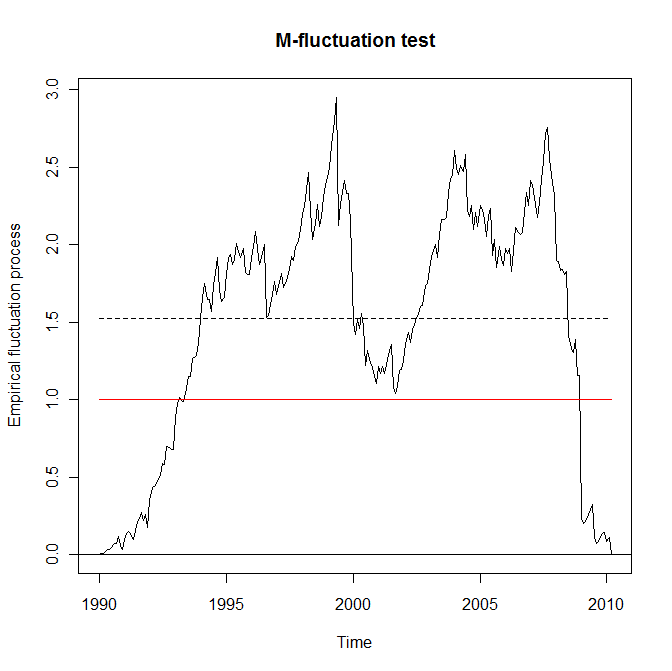
\includegraphics[width=80mm]{aut-meanL2BB.png}
\caption{Cram�r-von Mises test for Austria}
\end{figure}

Regarding the figure, we have two clear breaks, one in 1999 and another in 2008. [dating very unsure] The fxregimes procedure gives no breakdate. To give at least some intuition about the changes in variance [actually this is just scale, but can be adapted quickly] we forced 5 breaks into the Austrian inflation rates. 

\begin{figure}[h!tp]
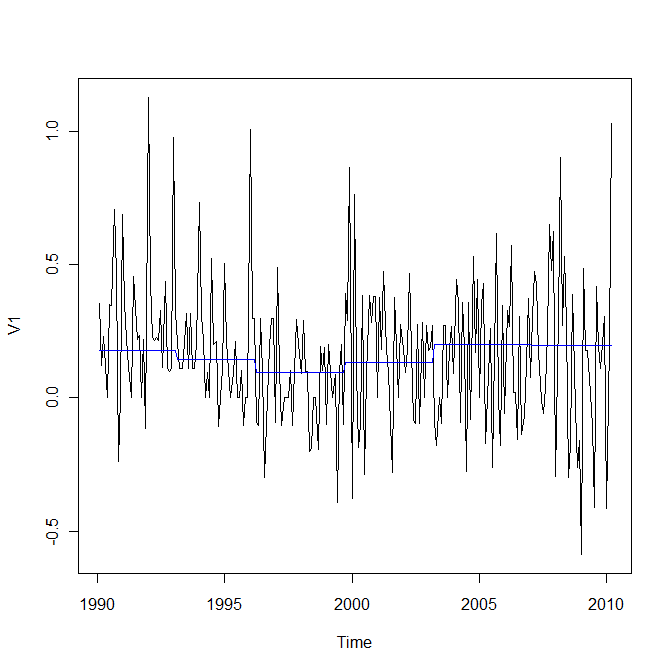
\includegraphics[width=80mm]{aut-morebreak.png}
\caption{Variance Estimation in Austrian Inflation Rates with 5 Breaks}
\end{figure}

Only with some phantasy we can se some slight V shape (a decline in inflation volatility up to 2000, then an increase). 




\subsection{Belgium}

Regarding the belgian inflation rates, all tests clearly indicate a break. 

\begin{figure}[h!tp]
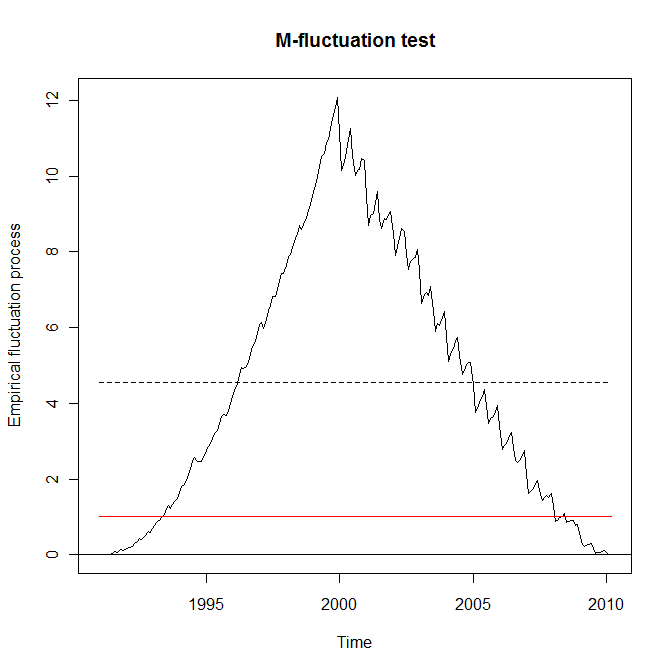
\includegraphics[width=80mm]{bel-meanL2BB.png}
\caption{Cram�r-von Mises test for Belgium}
\end{figure}

The fxregimes procedure indicates a breakpoint in December 2000.

%The impact of skewness: negative skew (rechtssteil), ie. higher values of y are more probable; positive skew (linkssteil): lower values of y are more probable
%so if it is the case like 6-2-1 we can say that the distribution gets less of a positive skew meaning a lower inflation on average (abkl�ren, sobald das mit den Momenten hinhaut)
%

\subsection{Italy}

In the italian case, there is clear evidence for two breaks. 


\begin{figure}[h!tp]
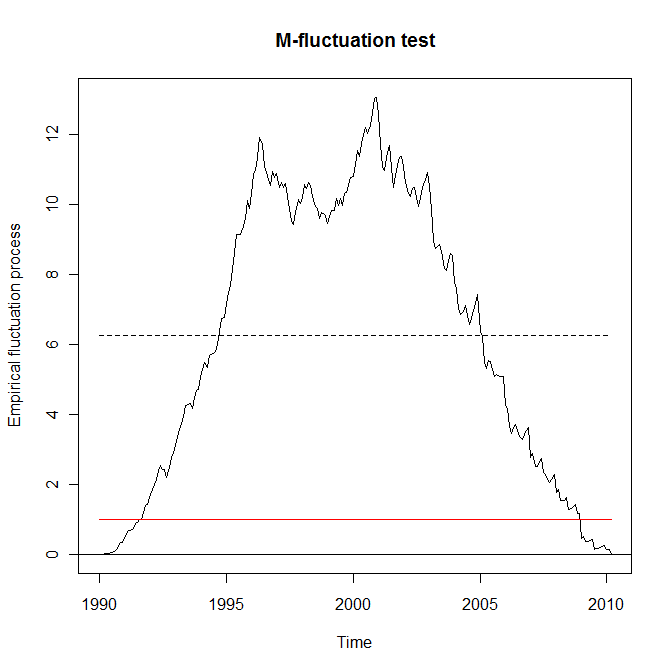
\includegraphics[width=80mm]{ita-meanL2BB.png}
\caption{Cram�r-von Mises test for Italy}
\end{figure}

If we compare the density of a whole and the denisties of the subsets of the data, we see a clear picture:

\begin{figure}[h!tp]
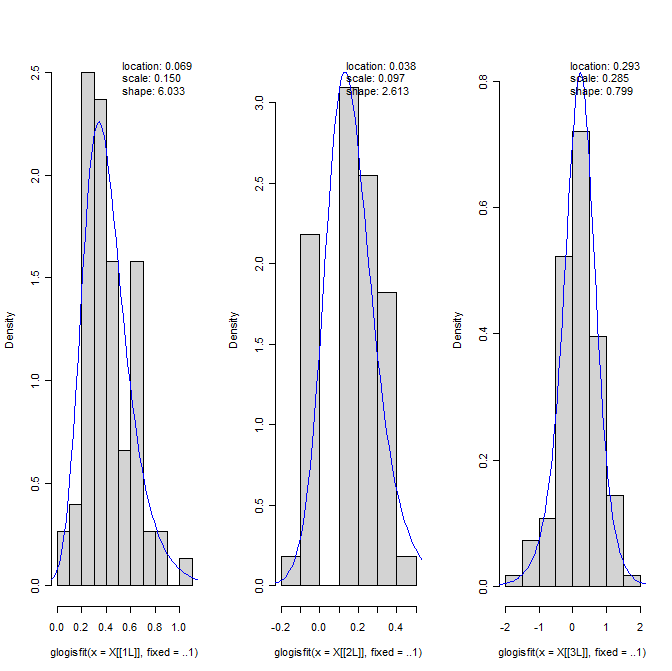
\includegraphics[width=80mm]{ita-split.png}
\caption{Parameters and Densities for subsamples}
\end{figure}


As we can see regarding the moments of the subsamples, we see a clear increase in variance (0.04, 0.01, 0.32), some smaller increase in the mean (0.41, 0.16, 0.18)  and a interesting increas in decrease in skewness (0.96, 0.71, $-$0.26), which means that lower values of the inflation rate are quickly becoming less probable. 



%\section{Ideas, Suggestions, Questions}
%
%Is there a method to get the dates in $"`plot(aut_gefp, functional=meanL2BB)"'$ (ie. return the date when we have the maximum value (or the two or more maximum values))? \\
%How to get more focus on variance ? \\
%How to force more than 5 breaks, so we end up with something as a "`smooth"' variance estimation. Good for graphical interpretation in the cases where there is no clear cut break. \\
%Use a GARCH model with a GL density, if considered useful \\
%If we find a break, how can we be sure that its the EMU whos responsible? The case if we find nothing is simpler, we can state that EMU had no effect (because otherwise we would see something, and the argument that EMU would be counteracted by something else is very very difficult to win) \\
%Goodness of fit test could produce a graph showing the fit in cdf and ecdf and some stars showing significance or a message.... 
%
%
%
%





\setstretch{1,3}



\newpage
\section{Literature}



\renewcommand*{\refname}{}
\bibliography{papers}
\begin{thebibliography}{99}
\bibliographystyle{apsr}




\end{document}